\documentclass[../TDE1-E2.tex]{subfiles}%

\begin{document}
\section[s]"2"{Association de générateurs~: calcul}

  \enonce{%
      Deux générateurs de tension ($E_1$, $r_1$) et ($E_2$, $r_2$) sont placés en
  parallèle l'un de l'autre. Ils alimentent une résistance $R_4$, également placée
  en parallèle sur les générateurs.
  }%

\QR{%
  Dessiner le schéma normalisé de ce montage et flécher les courants et
        les tensions. Exprimer alors l'intensité du courant qui circule dans $R_4$ et en déduire la tension aux bornes de $R_4$.
}{%
\begin{tcbraster}[raster columns=2, raster equal height=rows]
    \begin{tcn}(data){Schéma}
        \begin{center}
            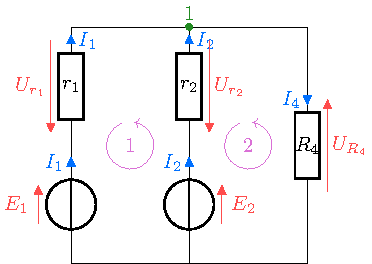
\includegraphics{assogen_parr-ldm}
        \end{center}
    \end{tcn}
    \begin{tcolorbox}[blankest, space to=\myspace]
        \begin{tcbraster}[raster columns=1]
            \begin{tcn}[add to natural height=\myspace](ques)'r'{Résultat attendu}
                On cherche $I_4$ puis $U_4 = R_4I_4$.
            \end{tcn}
            \begin{tcn}(tool)'r'{Outils}
                \begin{itemize}
                    \item LdM 1~: $I_4R_4 + I_1r_1 = E_1 \quad
                      \color{ForestGreen}(1)$~;
                    \item LdM 2~: $I_4R_4 + I_2r_2 = E_2 \quad
                      \color{ForestGreen}(2)$~;
                    \item LdN 1~: $I_1 + I_2 = I_4 \quad
                      \color{ForestGreen}(3)$.
                \end{itemize}
            \end{tcn} 
        \end{tcbraster}
    \end{tcolorbox}
\end{tcbraster}
\begin{tcbraster}[raster columns=7, raster equal height=rows]
    \begin{tcn}[raster multicolumn=3](ror){Approche méthodique}
        Notre but est de trouver une équation contenant $I_4$ et des valeurs
        connues, c'est-à-dire tout sauf $I_1, I_2$.
        \bigbreak
        L'équation \textcolor{ForestGreen}{(1)} peut nous aider~; on peut la
        transformer en remplaçant $I_1$ par $I_4-I_2$ grâce à
        \textcolor{ForestGreen}{(3)} pour avoir une équation
        \textcolor{ForestGreen}{(4)} avec $I_4$ et $I_2$.
        \bigbreak
        Mais comme \textcolor{ForestGreen}{(2)} nous permet d'isoler $I_2$ et de
        l'exprimer en fonction de $I_4$, en injectant cette expression dans
        \textcolor{ForestGreen}{(4)} on obtient une équation entre $I_4$ et les
        éléments du circuit. Question résolue !
    \end{tcn}
    \begin{tcn}[raster multicolumn=4](appl)'r'{Application}
        Avec \textcolor{ForestGreen}{(3)} dans \textcolor{ForestGreen}{(1)}~:
        \[I_4R_4 + (I_4-I_2)r_1 = E_1 \quad \color{ForestGreen}(4)\]
        En réexprimant \textcolor{ForestGreen}{(2)}~:
        \[I_2 = (E_2 - I_4R_4)/r_2\]
        En injectant \textcolor{ForestGreen}{(2)} dans
        \textcolor{ForestGreen}{(4)}~:
        \begin{align*}
            I_4(R_4+r_1) - (E_2-I_4R_4) \frac{r_1}{\color{brandeisblue}r_2}
                &= E_1\\
                \Leftrightarrow I_4(\textcolor{orange}{R_4} +
                                    \textcolor{red}{r_1})
                                    {\color{brandeisblue}r_2}
                                    -
                                    (E_2-I_4\textcolor{orange}{R_4})
                                    \textcolor{red}{r_1}
                &= E_1{\color{brandeisblue}r_2}\\
            \Leftrightarrow I_4(\textcolor{red}{r_1}
                                \textcolor{brandeisblue}{r_2} +
                                \textcolor{red}{r_1}\textcolor{orange}{R_4} +
                                \textcolor{brandeisblue}{r_2}\textcolor{orange}{R_4})
                &= E_1r_2 +E_2r_1
        \end{align*}
        Soit
        \[\boxed{I_4 = \frac{E_1r_2 + E_2r_1}{r_1r_2+r_1R_4+r_2R_4}} \quad
        \text{et} \quad \boxed{U_{R_4} = R_4\times I_4}\]
    \end{tcn}
\end{tcbraster}
}

\end{document}
